\documentclass[conference]{IEEEtran}

% =========================================================
% PLANTILLA LIGERA PARA OVERLEAF FREE
% Compilador recomendado: pdfLaTeX
% =========================================================
\renewcommand{\topfraction}{0.9}
\renewcommand{\bottomfraction}{0.8}
\renewcommand{\textfraction}{0.07}
\renewcommand{\floatpagefraction}{0.7}
\usepackage[utf8]{inputenc}
\usepackage[T1]{fontenc}
\usepackage[spanish,es-noshorthands]{babel}
\usepackage{lmodern}
\usepackage{microtype}
\usepackage[margin=1.8cm,columnsep=0.7cm]{geometry}
\usepackage{amsmath,amssymb}
\usepackage{graphicx}
\usepackage{algorithm}
\usepackage{algpseudocode}
\usepackage{booktabs}
\usepackage{verbatim}
\usepackage{array}
\usepackage{multirow}
\usepackage{xcolor}
\usepackage{caption}
\usepackage{float}
\usepackage{tikz}
\usepackage{url}
\usepackage{cite}
\usepackage{listings}
\usepackage{hyperref}
\usetikzlibrary{positioning,arrows.meta,fit,backgrounds}
\usepackage{pgfplots}
\pgfplotsset{compat=1.17}

\definecolor{CodeBackground}{HTML}{F4F6F7}
\definecolor{CodeKeyword}{HTML}{005F73}
\definecolor{CodeComment}{HTML}{6C757D}
\definecolor{CodeString}{HTML}{BB3E03}
% --- ELIMINADO: algorithm2e (incompatible con algorithm+algpseudocode) ---
% \usepackage[ruled,vlined,linesnumbered]{algorithm2e}
\captionsetup{font=small,labelfont=bf}
% --- El paquete 'algorithm' ya define el nombre en español vía babel; ---
% --- \SetAlgorithmName es opcional. Si lo quieres, deja solo esta línea: ---
\floatname{algorithm}{Algoritmo}
\renewcommand{\algorithmicrequire}{\textbf{Entrada:}}
\renewcommand{\algorithmicensure}{\textbf{Salida:}}
\setlength{\parskip}{0.2em}
\sloppy




% =========================================================
% DATOS DEL ARTÍCULO — EDITAR AQUÍ
% =========================================================
\title{\textbf{Diseño e implementación de un visor interactivo de ECG de multiples derivaciones con exportación de imágenes y evaluación del consumo de recursos}}

\author{
\IEEEauthorblockN{
Kevin Javier Gonzalez Luna,
Iván Felipe Maluche Suarez,
Angélica Pascagaza Vega
}
\IEEEauthorblockA{
\textit{Universidad Nacional de Colombia}\\
\textit{Sede Bogotá}\\
Bogotá D.C., Colombia\\
\{kegonzalezl, imaluche, apascagaza\}@unal.edu.co
}
}
\begin{document}

\maketitle

% =========================================================
% RESUMEN
% =========================================================

\begin{abstract}
Este documento presenta el diseño y posterior implementacion de un lector de señales ECG por medio de las estructuras de datos aprendidas a lo largo del curso, para esto el grupo se basa en diferentes papers y estudios que permitan comprender a fondo la lectura de estas señales con el fin de ser capaces de mostrarlas, leerlas adecuadamente y a partir de patrones poder predecir posibles afectaciones presentes en el corazon.
\end{abstract}

\begin{IEEEkeywords}
Medicina, Electro cardiograma, estructuras de datos, WFDB, PhysioNet, visualización interactiva, detección de QRS, Java, evaluación de rendimiento
algoritmos, instrumentos de medicion, Random Forest, prediccion.
\end{IEEEkeywords}

% =========================================================
% CONTENIDO
% =========================================================

\section{Introducción}

En el campo de la cardiologia debido a la complejidad y gravedad de las enfermades se hace de especial importancia el uso de herramientas capaces de leer y analizar datos clinicos de los pacientes de manera que se pueda advertir de posibles riesgos para su salud, sabiendo como esta tarea puede encontrar solucion en las estructuras de datos como grupo vemos de especial interes hacer uso de lo visto en el curso
para clasificar los datos clinicos de un paciente de forma que se puedan leer y analizar de manera eficiente por parte del personal de salud.

Para este fin nuestro proyecto abordara e implementara un algoritmo para la lectura, analisis y graficacion de señales ECG (obtenidas a base de un electrocardiograma) para ser capaces de entregar un reporte con posibles motivos de comportamientos anomalos por medio de algoritmos capaces de predecir patrones.

\subsection{Definicion del proyecto}
La idea central se basa en apoyarse de los temas que se han ido aprendiendo a lo largo del semestre sobre diferentes estructuras de datos para implementarlas en el manejo de los datos del ECG y detectar tanto propiedades como anomalias de este, esta metodologia permitira innovacion y replanteamiento de ideas a largo del proceso de desarrollo al a vez que la adicion de mejoras en cuanto a eficiencia y funcionamiento que facilmente pueden entrar tanto en el contexto del curso como del propio proyecto. 


\subsection{Objetivos}

\begin{itemize}
    \item \textbf{Ser capaz de leer registros de la base de datos MIT-BIH Arrhythmia Database (2 canales), PTBDB (15 canales) y PTB-XL(12 canales) incluyendo los archivos de registro y las anotaciones del cardiologo.} \cite{MIT-BIH} \cite{PhysioNet}
    \item \textbf{Hacer un uso activo de estructuras de datos vistas en el curso capaces de permitir una recepcion y envio eficiente de datos para el procesamiento y filtrado de informacion}
    \item \textbf{Implementar un algoritmo capaz de predecir casos a partir de modelos para entrenamiento de algoritmos, esto se hara por medio del uso de los random forest (los cuales son a su vez una implementacion de arboles de decision binarios)}
    \item \textbf{Entregar un resultado facil de leer para el cardiologo de manera que permita analizar los datos facilmente} 
\end{itemize}
\section{Estado del arte}
\subsection{Señales ECG y su análisis medico}
Como uno de los campos mas importantes de la medicina, el analisis del corazon es una de las areas de mayor necesidad de avance por lo vital de su papel dentro del funcionamiento en el cuerpo humano y lo sensible que este organo puede llegar a ser ante cambios.
\\
Por este motivo el campo del analisis de la señales producidas por el corazon (señales ECG) estan en una constante busqueda por metodos cada vez mas rapidos y precisos de manera que cada vez sea mas factible la identificacion de factores de riesgro criticos y por tanto el cuidado de la salud y vida de pacientes. La necesidad anteriormente descrita de este campo de la medicina en los ultimos años se le ha puesto especial interes gracias al crecimiento de la inteligencia artificial dentro de diferentes campos y su prometedor uso en la medicina para justamente ser capaces de identificar posibles comportamientos anomalos rapidamentes a partir de patrones analizados previamente. \cite{MtECG} 
\subsection{El formato WFDB}
Un registro WFDB consta de una cabecera de texto (\texttt{.hea}) y uno o varios archivos binarios de señal (\texttt{.dat}). Para cada señal, la cabecera declara el archivo, el formato de codificación, la ganancia (unidades ADC por unidad física), la línea de base, las unidades, la resolución, el valor inicial, el \emph{checksum} y una descripción~\cite{wfdb}. Distintos canales pueden residir en archivos distintos y con formatos distintos, por lo que ninguna propiedad debe suponerse común. La conversión a unidad física de la muestra digital $D_i$ de la señal $i$ es
\begin{equation}
V_i=\frac{D_i-B_i}{G_i},
\label{eq:conv}
\end{equation}
con $B_i$ la línea base y $G_i$ la ganancia. Las anotaciones de referencia se almacenan en archivos aparte (\texttt{.atr}) con un formato de palabras de 16 bits.

\subsection{Detección de QRS}
El algoritmo de Pan y Tompkins~\cite{pantompkins1985} es el método clásico de detección en tiempo real: filtrado paso banda, derivación, elevación al cuadrado, integración en ventana móvil y umbrales adaptativos sobre las estimaciones de nivel de señal y de ruido. Se adoptó aquí una variante expresada en segundos (y no en muestras) para que sea independiente de la frecuencia de muestreo.

\subsection{Medición de recursos en la JVM}
Java ofrece \texttt{ThreadMXBean}, con el tiempo de CPU del hilo actual, y, en las implementaciones que lo soportan, la extensión \texttt{com.sun.management.OperatingSystemMXBean}, con la CPU total del proceso~\cite{oraclejmx}. No existe una API portable para separar el tiempo de CPU de usuario y de sistema del proceso; en Linux se puede leer \texttt{/proc/self/stat}. Del mismo modo, \texttt{Runtime.totalMemory()-freeMemory()} mide el heap utilizado y no la memoria física del proceso. Estas diferencias condicionan el diseño del módulo de rendimiento (Sección~\ref{sec:rend}).

\subsection{Random Forest}
Dentro de las implementaciones de las estructuras de datos y dentro del marco de la inteligencia artificial existe un sistema conformado por un tipo de arboles para realizar un modelo de aprendizaje capaz de realizar predicciones, a este modelo se le conoce como random forest.
\\
Como su nombre indica el modelo se conforma por un conjunto de arboles siendo de este caso arboles de decision, cada uno de estos arboles a base de un algoritmo que identifica los valores por umbrales de decision guarda una proporcion de las muestras en sus hojas. Cada uno de estos arboles aportara al sistema una prediccion que puede ser o no sesgada pero que en cualquier caso gracias a los demas arboles permitira una prediccion aproximada y confiable. \cite{RF}
\\
\textbf{Pd: Para comprender mas a fondo el funcionamiento de estos arboles se puede consultar el documento RandomForest.pdf ubicado en la carpeta anexos}
\section{requerimientos de la implementacion}
\label{sec:metodologia}

Debido a lo complejo y especializado que puede llegar a ser la medicion de señales ECG el proyecto tiene que cumplir con ciertos parametros especifocs que sin un correcto desempeño impedira el desarrollo adecuado de la implementacion.
\\
Tomando esto en cuenta el algoritmo debe ser capaz de:

\begin{itemize}
 \item Ser capaz de leer los archivos de la base de datos MIT (especificamente los archivos .hea, los cuales contienen la informacion necesaria para el analisis) \cite{MIT-BIH}
 \item Organizar los datos de manera que puedan ser facilmente leidos y manejados por las estructuras de datos
 \item Graficar los datos de manera que sean entendibles
 \item Filtrar ruido para obtener mejores resultados en las propiedades de la señal.
 \item Predecir posibles complicaciones a base del analisis de las señales presentadas.
\end{itemize}

\section{Diseño y arquitectura de la solucion}
\label{sec:diseño}

\subsection{Orden del proyecto del proyecto}
Dentro de la carpeta src disponible junto con este documento se encuentra la carpeta main, que contiene la carpeta java que a su vez contiene la carpeta ecg, dentro de esta se encuentra los aspectos relevantes de nuestro algoritmo:
\begin{itemize}
    \item \textbf{exportacion:} Contiene los archivos necesarios para convertir los resultados graficos obtenidos a formato PNG, incluye soporte para canales seleccionados y de la vista exacta actual.
    \item \textbf{interfaz:} Contiene todos los archivos que definen la forma del programa y su interaccion con el usuario
    \item \textbf{lectura:} Dentro de esta carpeta se encuentra el conjunto de programas que hacen posible la lectura de los archivos del ECG.
    \item \textbf{ml:} Dentro de la carpeta se encuentran los archivos pertenencientes al Random forest junto con algunos ejemplos y las estructuras implementadas para el proyecto (Dynarray,Cqueue, heaps, etc) un readme con una explicacion, esto se hace con el fin de comprender esta estructura que a diferencia de las demas usadas es de especial complejidad.
    \item \textbf{modelo:} Contiene el codigo encargado de entre otras tareas dar los resultados, identificar las anotaciones, etc.
    \item \textbf{procesamiento:} Como su nombre indica dentro de esta carpeta se encuentran los diferentes archivos que permiten al codigo procesar la informacion obtenida de los registros y las prediccions.
    \item \textbf{rendimiento:} Los archivos dentro permiten el funcionamiento adecuado de la pestaña de rendimiento dentro del programa.
    \item \textbf{utilidades:} Contiene funciones usadas para facilitar el desarrollo del algoritmo en otras secciones del codigo.
    \item \textbf{Main.java:} Archivo principal del programa, es en donde sucede todo el loop principal de operacion.
\end{itemize}

\subsection{Loop basico de la implementacion}
Inicialmente el programa realiza una comprobacion inicial con la carpeta test presente al mismo nivel de la carpeta main, hecho esto usa las diferentes subcarpetas explicadas anteriormente para componer el programa y ser capaz de manejar archivos de ECG.
\subsection{Futuros aspectos a implementar}
Tomando en cuenta lo alcanzado en esta segunda etapa de la implementacion y como se avanzo hasta llegar a un resultado bastante considerable el grupo esta a la espera de los temas del tercer corte de forma que se pueda valorar mas estructuras para implementacion o determinar el resultado actual como suficientemente adecuado.
\subsection{Arquitectura}
%=====================================================================
La aplicación se organiza en tres subsistemas (lectura y procesamiento, visualización y exportación, evaluación de rendimiento) soportados por ocho paquetes (Fig.~\ref{fig:arq}). La Tabla~\ref{tab:codigo} resume su tamaño.

\begin{figure*}[t]
\centering
\begin{tikzpicture}[
  caja/.style={draw,rounded corners=2pt,minimum height=0.8cm,minimum width=2.5cm,font=\small,align=center,fill=blue!6},
  cajaA/.style={draw,rounded corners=2pt,minimum height=0.8cm,minimum width=2.5cm,font=\small,align=center,fill=green!8},
  cajaB/.style={draw,rounded corners=2pt,minimum height=0.8cm,minimum width=2.5cm,font=\small,align=center,fill=orange!10},
  flecha/.style={-{Stealth[length=2mm]},thick}]
  \node[cajaA] (arch) {Archivos\\\texttt{.hea}/\texttt{.dat}/\texttt{.atr}};
  \node[caja,right=0.9cm of arch] (lect) {\texttt{lectura}};
  \node[caja,right=0.9cm of lect] (mod) {\texttt{modelo}\\{\scriptsize RegistroECG, ConfiguracionVista}};
  \node[caja,right=0.9cm of mod] (proc) {\texttt{procesamiento}};
  \node[caja,below=1.0cm of mod] (vis) {\texttt{visualizacion}\\{\scriptsize RenderizadorECG}};
  \node[caja,left=0.9cm of vis] (exp) {\texttt{exportacion}\\{\scriptsize PNG}};
  \node[caja,right=0.9cm of vis] (int) {\texttt{interfaz}\\{\scriptsize Swing, controlador}};
  \node[cajaB,below=1.0cm of vis] (rend) {\texttt{rendimiento}\\{\scriptsize medidores, PDF}};
  \node[cajaA,right=0.9cm of int] (usr) {Usuario};
  \draw[flecha] (arch)--(lect);
  \draw[flecha] (lect)--(mod);
  \draw[flecha] (mod)--(proc);
  \draw[flecha] (mod)--(vis);
  \draw[flecha] (vis)--(exp);
  \draw[flecha] (int)--(vis);
  \draw[flecha] (usr)--(int);
  \draw[flecha,dashed] (rend)--(vis);
  \draw[flecha,dashed] (rend.east) -| (int.south);
  \draw[flecha,dashed] (rend.west) -| ([xshift=-0.6cm]exp.south);
  \node[font=\scriptsize,below=0.15cm of rend] {discontinua: mide las operaciones de la capa};
\end{tikzpicture}
\caption{Arquitectura modular. Las flechas continuas indican flujo de datos; las discontinuas, medición de rendimiento. La capa \texttt{utilidades} (rutas, formatos, generador sintético) es transversal.}
\label{fig:arq}
\end{figure*}

\begin{table}[t]
\centering\small
\caption{Tamaño del código (líneas Java).}
\label{tab:codigo}
\begin{tabular}{@{}lrr@{}}
\toprule
Paquete & Archivos & Líneas \\
\midrule
\texttt{modelo}        & 9  & 441 \\
\texttt{lectura}       & 13 & 762 \\
\texttt{procesamiento} & 9  & 488 \\
\texttt{visualizacion} & 15 & 921 \\
\texttt{exportacion}   & 8  & 313 \\
\texttt{rendimiento}   & 9  & 975 \\
\texttt{interfaz}      & 12 & 1\,193 \\
\texttt{utilidades}    & 6  & 257 \\
\texttt{ml}   & 8  & 1\,040 \\
\texttt{Estructuras}   & 5  & 651 \\
\texttt{Main}          & 1  & 95 \\
\midrule
Total (código)         & 82 & 7\,136 \\
\bottomrule
\end{tabular}
\end{table}

Se establecieron cuatro principios de diseño: (i) el número de canales lo dicta la cabecera (listas dinámicas, sin matrices de tamaño fijo); (ii) cada canal conserva sus metadatos, incluidos archivo, ganancia y línea base; (iii) la configuración de vista es el único estado compartido entre el visor y los exportadores; y (iv) las interacciones (zoom, desplazamiento) modifican únicamente esa configuración, nunca las muestras.

\section{Implementación}
%=====================================================================
\subsection{Lectura de registros WFDB}
El flujo de carga es: cabecera $\rightarrow$ validación $\rightarrow$ decodificación por archivo $\rightarrow$ conversión de unidades $\rightarrow$ \texttt{RegistroECG}. El analizador de cabeceras interpreta cada línea de señal con expresiones regulares para el formato (\texttt{formato[xN][:skew][+offset]}) y la ganancia (\texttt{ganancia[(baseline)][/unidades]}); si no hay línea base explícita se adopta el valor ADC cero. Los registros multisegmento se rechazan con un mensaje explícito.

Las señales se agrupan por archivo y cada grupo se decodifica con la implementación correspondiente a su formato. El formato 16 son enteros de 16 bits con signo \emph{little-endian}. En el formato 212, dos muestras de 12 bits comparten tres bytes; numerando las muestras intercaladas con $k=0,1,\dots$ y siendo $b$ el desplazamiento del grupo de tres bytes $(b_0,b_1,b_2)$ al que pertenece:
\begin{equation}
v_k=\begin{cases}
b_0+256\,(b_1\ \&\ \mathrm{0x0F}) & k\ \text{par},\\
b_2+16\,(b_1\ \&\ \mathrm{0xF0}) & k\ \text{impar},
\end{cases}
\end{equation}
con extensión de signo de 12 bits. En el formato 8 se acumulan diferencias con signo a partir del valor inicial de cada señal; los formatos 24 y 32 son enteros de 3 y 4 bytes. Este diseño por intercalado global permite cualquier número de canales, incluido un número impar con muestra final a medias.

La conversión \eqref{eq:conv} se realiza en una única clase. Las unidades de tensión se normalizan a mV ($\mu$V, V, nV); las no eléctricas se conservan. El valor reservado $-32768$ del formato 16 se transforma en \texttt{NaN} (muestra inválida), que el renderizador representa como un hueco. Un registro sin ganancia declarada se rechaza en lugar de aplicar un valor supuesto. Finalmente, la suma módulo $2^{16}$ de cada señal se compara con el \emph{checksum} de la cabecera para detectar errores de decodificación; una discrepancia genera una advertencia, pero no bloquea la carga.


\subsection{Procesamiento de señal}

El procesamiento se organiza en dos etapas encadenadas sobre cada derivación $x[n]$ de frecuencia $f_s$: (i) \textbf{detección de complejos QRS} y (ii) \textbf{clasificación de cada latido} en una de las cuatro clases AAMI (N, S, V, F) mediante un \emph{Random Forest}. Todo el cómputo es independiente de $f_s$: las ventanas se definen en segundos y se convierten a muestras con $\lfloor w f_s \rceil$.

\subsubsection{Detección QRS (Pan-Tompkins con media móvil)}

El detector procesa cada derivación con ventanas definidas en segundos:
\begin{align}
y_1[n]&=x[n]-\mathrm{MM}_{0{,}20 f_s}(x)[n],\quad y_2=\mathrm{MM}_{0{,}025 f_s}(y_1),\\
d[n]&=\tfrac{1}{8}\bigl(2y_2[n{+}2]+y_2[n{+}1]-y_2[n{-}1]-2y_2[n{-}2]\bigr),\\
m&=\mathrm{MM}_{0{,}15 f_s}\!\bigl(d^{2}\bigr),
\end{align}
donde $\mathrm{MM}_w$ es una media móvil centrada de $w$ muestras calculada en $O(n)$ con sumas acumuladas. Sobre $m$ se buscan máximos locales y se mantienen las estimaciones de nivel de señal ($S$) y de ruido ($N$) con
\begin{align}
S&\leftarrow \tfrac18 m_i+\tfrac78 S,\qquad N\leftarrow \tfrac18 m_i+\tfrac78 N,\\
\theta&=N+\tfrac14(S-N).
\end{align}
Un candidato se acepta si $m_i>\theta$ y han pasado más de 0,2\,s desde el latido previo (periodo refractario); si cae a menos de 0,36\,s del previo y su pendiente máxima $|d|$ es menor que la mitad de la del latido previo, se trata como onda T. El pico se refina al máximo de $|y_2|$ en $\pm 0{,}08$\,s, lo que permite detectar R negativas (p.~ej. aVR). La pendiente máxima en ventana se calcula en $O(n)$ con un \emph{deque} monótono (\texttt{maxAbsVentana}), evitando el coste $O(n\cdot w)$ del cálculo ingenuo. No se implementó la búsqueda hacia atrás de latidos perdidos.

\subsubsection{Fusión de canales por consenso}

El detector se ejecuta por derivación y los resultados se combinan por consenso (Alg.~\ref{alg:fusion}): los candidatos de todos los canales se ordenan, se agrupan cuando la distancia entre consecutivos es inferior a 0,1\,s y se aceptan los grupos con al menos $\lceil n/2\rceil$ canales distintos, usando la mediana como posición del latido. A partir de los latidos se calculan los intervalos $RR_i=(n_{i+1}-n_i)/f_s$, la frecuencia instantánea $FC_i=60/RR_i$ y las medidas SDNN y RMSSD.

\begin{algorithm}[t]
\small
\caption{Fusión de detecciones por consenso}
\label{alg:fusion}
\begin{algorithmic}[1]
\Require detecciones por canal, ventana $w$, votos mínimos $v$
\Ensure lista de latidos fusionados
\State $C\leftarrow$ todos los pares (índice, canal), ordenados por índice
\State $g\leftarrow\emptyset$
\ForAll{$c\in C$}
  \If{$g\neq\emptyset$ \textbf{y} $c.\mathrm{indice}-\mathrm{ultimo}(g).\mathrm{indice}>w f_s$}
    \State cerrar($g$); $g\leftarrow\emptyset$
  \EndIf
  \State añadir $c$ a $g$
\EndFor
\State cerrar($g$) \Comment{acepta si canales distintos $\ge v$; guarda la mediana}
\end{algorithmic}
\end{algorithm}

\subsubsection{Extracción de características por latido}

Cada latido detectado en la posición $p$ se describe con \textbf{257 números} (vector de características $\phi\in\mathbb{R}^{257}$), calculados por \texttt{Caracteristicas.extraer}:

\textbf{Forma del latido (252 valores).} Sea $c=\mathrm{recentrar}(x,p)$ el pico R refinado al mayor $|x-\mathrm{mediana}|$ en $\pm 50$\,ms. La ventana de forma es
\begin{equation}
f_j \;=\; x[c-90+j]-\tilde{x},\qquad j=0,\dots,251,
\end{equation}
donde $\tilde{x}$ es la mediana de $x$ en $[c-90,\,c+162)$ y se usan 90 muestras antes y 162 desde el pico (a 360\,Hz: 0,25\,s y 0,45\,s). Restar la mediana elimina la línea base.

\textbf{Ritmo (5 valores).} Con $d_i=c_i-c_{i-1}$ el número de muestras entre latidos consecutivos y $\overline{d}_i$ la media de los últimos 10 $d$:
\begin{equation}
\phi_{252..256}=\Bigl(\tfrac{d_{i-1}}{f_s},\;\tfrac{d_{i+1}}{f_s},\;\tfrac{\overline{d}_i}{f_s},\;\tfrac{d_{i-1}}{\overline{d}_i},\;\tfrac{d_{i+1}}{\overline{d}_i}\Bigr).
\end{equation}
Estos cinco valores capturan latidos que llegan antes o después de lo normal (extrasístoles, pausas). Si la ventana de 252 muestras no cabe en la señal (extremos del registro), el latido se descarta para clasificación pero \textbf{sí} cuenta para los intervalos RR.

\subsubsection{Clasificación con Random Forest}

El clasificador es un \textbf{Random Forest de $T$ árboles de decisión} implementado sin librerías externas (\texttt{BosqueSimple}, \texttt{ArbolDesicion}). Cada árbol $t$ se entrena con un \textbf{bootstrap} de las muestras de DS1 (filas sorteadas con repetición) y, en cada nodo, considera solo un subconjunto aleatorio de $k=\lfloor\sqrt{257}\rfloor\approx 16$ características.

\textbf{Criterio de corte.} En un nodo con muestras $\mathcal{S}$, la \textbf{entropía de Shannon} de las clases es
\begin{equation}
H(\mathcal{S})=-\sum_{c=1}^{4} p_c\log_2 p_c,\qquad p_c=\frac{|\{m\in\mathcal{S}:y_m=c\}|}{|\mathcal{S}|},
\end{equation}
y la \textbf{ganancia de información} de un corte ``$\phi_j<\theta$'' es
\begin{equation}
\Delta H(\mathcal{S},j,\theta)=H(\mathcal{S})-\frac{|\mathcal{S}_{\mathrm{izq}}|}{|\mathcal{S}|}H(\mathcal{S}_{\mathrm{izq}})-\frac{|\mathcal{S}_{\mathrm{der}}|}{|\mathcal{S}|}H(\mathcal{S}_{\mathrm{der}}).
\end{equation}
Para cada característica candidata $j$ se fija $\theta=\overline{\phi_j}$ (la media de esa característica en el nodo) y se elige el par $(j^\star,\theta^\star)$ de mayor $\Delta H$. El nodo se parte en $\mathcal{S}_{\mathrm{izq}}=\{m:\phi_{m,j^\star}<\theta^\star\}$ y $\mathcal{S}_{\mathrm{der}}$ el resto, y se repite recursivamente hasta que el grupo es puro, tiene menos de $\ell_{\min}$ muestras, o ninguna partición lo separa. Cada hoja guarda la \textbf{distribución empírica de clases} $p=(p_N,p_S,p_V,p_F)$ de sus muestras.

\textbf{Predicción (voto blando).} Para un latido nuevo con vector $\phi$, cada árbol $t$ devuelve la distribución $p^{(t)}(\phi)$ de la hoja alcanzada. El bosque promedia:
\begin{equation}
\hat{p}(\phi)=\frac{1}{T}\sum_{t=1}^{T}p^{(t)}(\phi),\qquad \hat{y}=\arg\max_{c\in\{N,S,V,F\}}\hat{p}_c(\phi).
\end{equation}
La doble aleatoriedad (bootstrap de filas + subconjunto de características por nodo) descorrelaciona los árboles y reduce la varianza del ensamble frente a un árbol único. Con semilla fija el bosque es reproducible bit a bit.

\textbf{Fusión entre derivaciones.} Si el registro tiene varias derivaciones, cada latido se clasifica en todas ellas (cuando la ventana cabe) y se promedian las distribuciones $\hat{p}^{(d)}$ de las derivaciones votantes antes de aplicar el $\arg\max$; si solo una derivación aporta, se usa directamente.

\begin{algorithm}[t]
\small
\caption{Entrenamiento de un árbol del bosque (nodo $\mathcal{S}$)}
\label{alg:arbol}
\begin{algorithmic}[1]
\Require muestras $\mathcal{S}$, nº clases $C{=}4$, características por nodo $k$, mínimo de hoja $\ell_{\min}$
\Ensure nodo del árbol
\If{$|\mathcal{S}|<\ell_{\min}$ \textbf{o} todas las $y_m$ iguales}
  \State \Return hoja con distribución $p_c=|\{m:y_m=c\}|/|\mathcal{S}|$
\EndIf
\State $\mathcal{J}\leftarrow$ subconjunto aleatorio de $k$ características
\State $(j^\star,\theta^\star)\leftarrow\arg\max_{j\in\mathcal{J},\,\theta=\overline{\phi_j}}\Delta H(\mathcal{S},j,\theta)$
\State partir $\mathcal{S}$ en $\mathcal{S}_{\mathrm{izq}},\mathcal{S}_{\mathrm{der}}$ por $(j^\star,\theta^\star)$
\If{$\mathcal{S}_{\mathrm{izq}}=\emptyset$ \textbf{o} $\mathcal{S}_{\mathrm{der}}=\emptyset$}
  \State \Return hoja con distribución de $\mathcal{S}$
\EndIf
\State \Return nodo interno $(j^\star,\theta^\star)$ con hijos
  \textsc{Árbol}$(\mathcal{S}_{\mathrm{izq}})$ y \textsc{Árbol}$(\mathcal{S}_{\mathrm{der}})$
\end{algorithmic}
\end{algorithm}

\subsubsection{Validación de detección y clasificación}

La validación de la \textbf{detección} compara detecciones y referencia con emparejamiento uno a uno y tolerancia $\tau$, calculando verdaderos positivos (TP), falsos positivos (FP) y falsos negativos (FN):
\begin{equation}
Se=\frac{TP}{TP+FN},\quad P^{+}=\frac{TP}{TP+FP},\quad F_1=\frac{2\,Se\,P^{+}}{Se+P^{+}},
\end{equation}
además del error temporal medio $|\Delta t|$ de los latidos emparejados. La validación de la \textbf{clasificación} usa la matriz de confusión $4\times4$ $M[\text{real}][\text{predicho}]$ y, por clase $c$ (uno contra el resto), calcula
\begin{align}
P_c&=\frac{M_{cc}}{\sum_i M_{ic}},\qquad
R_c=\frac{M_{cc}}{\sum_j M_{cj}},\\
F1_c&=\frac{2P_cR_c}{P_c+R_c},\qquad
\text{F1}_{\text{macro}}=\frac14\sum_c F1_c.
\end{align}


\subsubsection{Flujo completo (pipeline)}
\begin{figure}[t]
\centering
\begin{tikzpicture}[
  caja/.style={draw,rounded corners=2pt,minimum height=0.65cm,minimum width=6.3cm,
               font=\scriptsize,align=center,fill=blue!6,inner sep=2pt},
  cajaA/.style={draw,rounded corners=2pt,minimum height=0.65cm,minimum width=6.3cm,
                font=\scriptsize,align=center,fill=green!8,inner sep=2pt},
  cajaB/.style={draw,rounded corners=2pt,minimum height=0.65cm,minimum width=6.3cm,
                font=\scriptsize,align=center,fill=orange!10,inner sep=2pt},
  flecha/.style={-{Stealth[length=1.8mm]},thick},
  etiq/.style={font=\tiny,above,midway,align=center}]

  \node[cajaA] (reg)  {Registro WFDB (\texttt{.hea}/\texttt{.dat}/\texttt{.atr})};
  \node[caja,below=0.20cm of reg]  (det)  {\texttt{DetectorPanTompkins.detectar}$(x_d,f_s)$};
  \node[caja,below=0.20cm of det]  (fus)  {\texttt{FusionDetecciones.fusionar}$(\dots,\lceil n/2\rceil)$};
  \node[caja,below=0.20cm of fus]  (car)  {\texttt{Caracteristicas.extraer}$(x,\text{pos.})$};
  \node[cajaB,below=0.20cm of car] (bos)  {\texttt{BosqueSimple.predecirDistribucion}$(\phi)$};
  \node[caja,below=0.20cm of bos]  (arg)  {$\arg\max_c\,\hat{p}_c(\phi)\;\to$\; AAMI ($N/S/V/F$)};
  \node[cajaA,below=0.20cm of arg] (met)  {\texttt{Metricas.matrizConfusion}\,/\,\texttt{reporte}};

  \draw[flecha] (reg) -- node[etiq] {índices $R$} (det);
  \draw[flecha] (det) -- node[etiq] {latidos} (fus);
  \draw[flecha] (fus) -- node[etiq] {$\phi\in\mathbb{R}^{257}$} (car);
  \draw[flecha] (car) -- node[etiq] {$\hat{p}$} (bos);
  \draw[flecha] (bos) -- node[etiq] {$\hat y$} (arg);
  \draw[flecha] (arg) -- node[etiq] {} (met);
\end{tikzpicture}
\caption{Flujo completo de procesamiento: detección QRS por derivación, fusión por consenso, extracción de las 257 características, clasificación con el bosque aleatorio (voto blando) y validación opcional contra la referencia.}
\label{fig:pipeline}
\end{figure}

\subsubsection{Parámetros e implementación}

\begin{table}[t]
\centering
\footnotesize
\setlength{\tabcolsep}{3pt}
\begin{tabular}{@{}lcc@{}}
\toprule
Parámetro & Valor & Archivo \\
\midrule
Árboles del bosque $T$ & 25 & \texttt{Bosque\-Simple} \\
Caract. por nodo $k$ & $\lfloor\sqrt{257}\rfloor{=}16$ & \texttt{Bosque\-Simple} \\
Mín. de muestras por hoja $\ell_{\min}$ & 20 & \texttt{Arbol\-Desicion} \\
Semilla del azar & 0 & \texttt{Muestreo} \\
Ventana de fusión & 0,10\,s & \texttt{Analizador\-ECG} \\
Tolerancia de validación $\tau$ & 0,15\,s & \texttt{Validador\-Deteccion} \\
\bottomrule
\end{tabular}
\caption{Hiperparámetros del detector y del clasificador.}
\label{tab:parametros}
\end{table}

El dataset de entrenamiento (DS1, 22 registros de MIT-BIH) se construye leyendo los WFDB con \texttt{Datos.construir} y se cachea en texto (\texttt{DSV1}) para no releerlos en cada arranque; el bosque entrenado se serializa en formato \texttt{RFV1} (recorrido en preorden, una línea por nodo) mediante \texttt{BosqueSimple.guardar}/\texttt{cargar}, lo que permite reutilizarlo sin re-entrenar. Las estructuras auxiliares (\texttt{DynamicArray}, \texttt{CircularQueue}, \texttt{MovingMean}, \texttt{MinHeap}) están implementadas a mano en \texttt{ecg.ml.estructuras}, sin depender de las colecciones de \texttt{java.util} para el núcleo del algoritmo.

% =====================================================================
% Referencias sugeridas (añádelas a tu .bib o a la bibliografía)
% =====================================================================


\subsection{Motor de dibujo}
El \texttt{RenderizadorECG} recibe un registro, una \texttt{ConfiguracionVista} y una superficie, sin conocer ventanas ni controles. Cada derivación visible ocupa una celda; la ventana temporal $[t_0,t_1]$ se ajusta al ancho $W$ de la celda y la amplitud se escala con la ganancia vertical $g_v$ (mm/mV) y la resolución $\rho$ (píxeles/mm):
\begin{equation}
x(t)=x_0+\frac{t-t_0}{t_1-t_0}W,\qquad
y(v)=y_c-g_v\,\rho\,v .
\end{equation}
La cuadrícula se dibuja en unidades de tiempo y tensión (0,04\,s y 0,1\,mV por cuadro pequeño; 0,2\,s y 0,5\,mV por cuadro grande) y se omiten los trazos con separación inferior a 3 o 6 píxeles. Cuando hay más de dos muestras por columna de píxeles, la señal se dibuja como envolvente mínimo/máximo, lo que acota el coste de repintado por la anchura de la celda y no por la longitud de la ventana. Las distribuciones (cuadrícula $3\times4$, vertical, individual y automática) se calculan con reparto entero para evitar huecos.

La impresión estándar calcula el tamaño de la imagen para que la calibración sea exacta: el ancho de cada celda es $T\cdot 25\cdot\rho$ píxeles para una ventana de $T$ segundos, y su alto $40\,\rho$ ($\pm2$\,mV a 10\,mm/mV). El visor interactivo traduce eventos de ratón y teclado (rueda: zoom horizontal con el instante bajo el cursor fijo; Ctrl+rueda: zoom vertical; arrastre: desplazamiento; Mayús+arrastre: selección de intervalo) en cambios sobre la configuración, tras lo cual repinta.

\begin{figure}[h!]
\centering
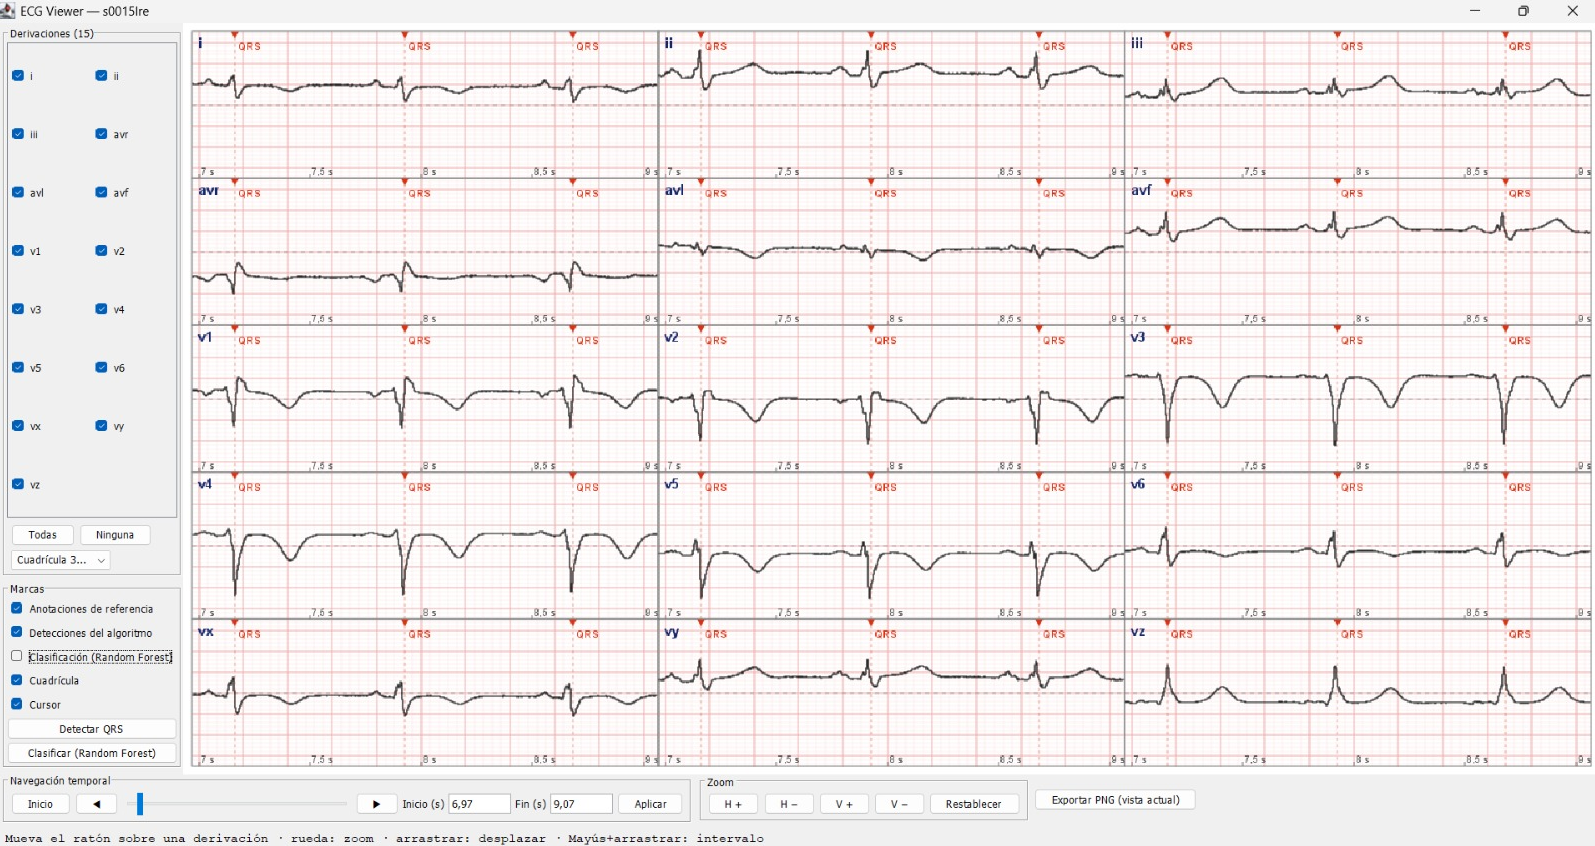
\includegraphics[width=0.44\textwidth]{images/estandar.png}
\caption{Impresión estándar de un registro de la base de datos de PTB Diagnostic ECG Database de 15 derivaciones (distribución $3\times4$, 5\,s, 25\,mm/s y 10\,mm/mV) con detección QRS (triángulos rojos). Imagen generada por la propia aplicación.}
\label{fig:estandar}
\end{figure}

\subsection{Exportación}
Todas las exportaciones heredan de una clase base que dibuja con el mismo \texttt{RenderizadorECG}. Se ofrecen cuatro variantes: impresión estándar, personalizada (derivaciones, intervalo, tamaño, escalas y anotaciones), vista actual (copia de la configuración vigente) y registro completo dividido en páginas de duración fija, para no comprimir registros largos en una sola imagen. Las copias de configuración eliminan el estado de inspección (cursor, selección) para que no aparezca en las impresiones, y se rechazan imágenes de más de $1{,}2\times10^{8}$ píxeles.

\subsection{Medición de rendimiento}
\label{sec:rend}
El \texttt{MonitorRendimiento} inicia una medición antes de cada operación y la cierra después, también si la operación falla; admite operaciones anidadas, registrando su profundidad para no sumar dos veces su coste en los totales. Cada medición combina tres medidores:
\begin{itemize}
  \item \textbf{Tiempo:} diferencia de \texttt{System.nanoTime()}; es tiempo de pared y por tanto incluye esperas.
  \item \textbf{Memoria:} heap usado al inicio y al final, máximo muestreado cada 5\,ms por un hilo auxiliar (una cota inferior del pico real), memoria reservada por la JVM y, en Linux, la memoria residente (RSS) de \texttt{/proc/self/status}.
  \item \textbf{CPU:} nivel portable (CPU del hilo y CPU total del proceso) y nivel específico del sistema operativo (usuario y sistema del proceso desde \texttt{/proc/self/stat}, suponiendo 100 ticks/s). Las magnitudes no disponibles se marcan como tales y nunca se obtienen restando fuentes de distinto origen.
\end{itemize}
El informe PDF (Apache PDFBox~\cite{pdfbox}) contiene la información de la ejecución, las métricas globales, la tabla por operación (con media, mínimo y máximo si hay repeticiones), tres gráficos generados con Java2D, información de aciertos del Random Forest y un apartado de observaciones con las limitaciones de medida. Se genera bajo demanda y no en cada interacción.
\begin{figure}[h!]
\centering
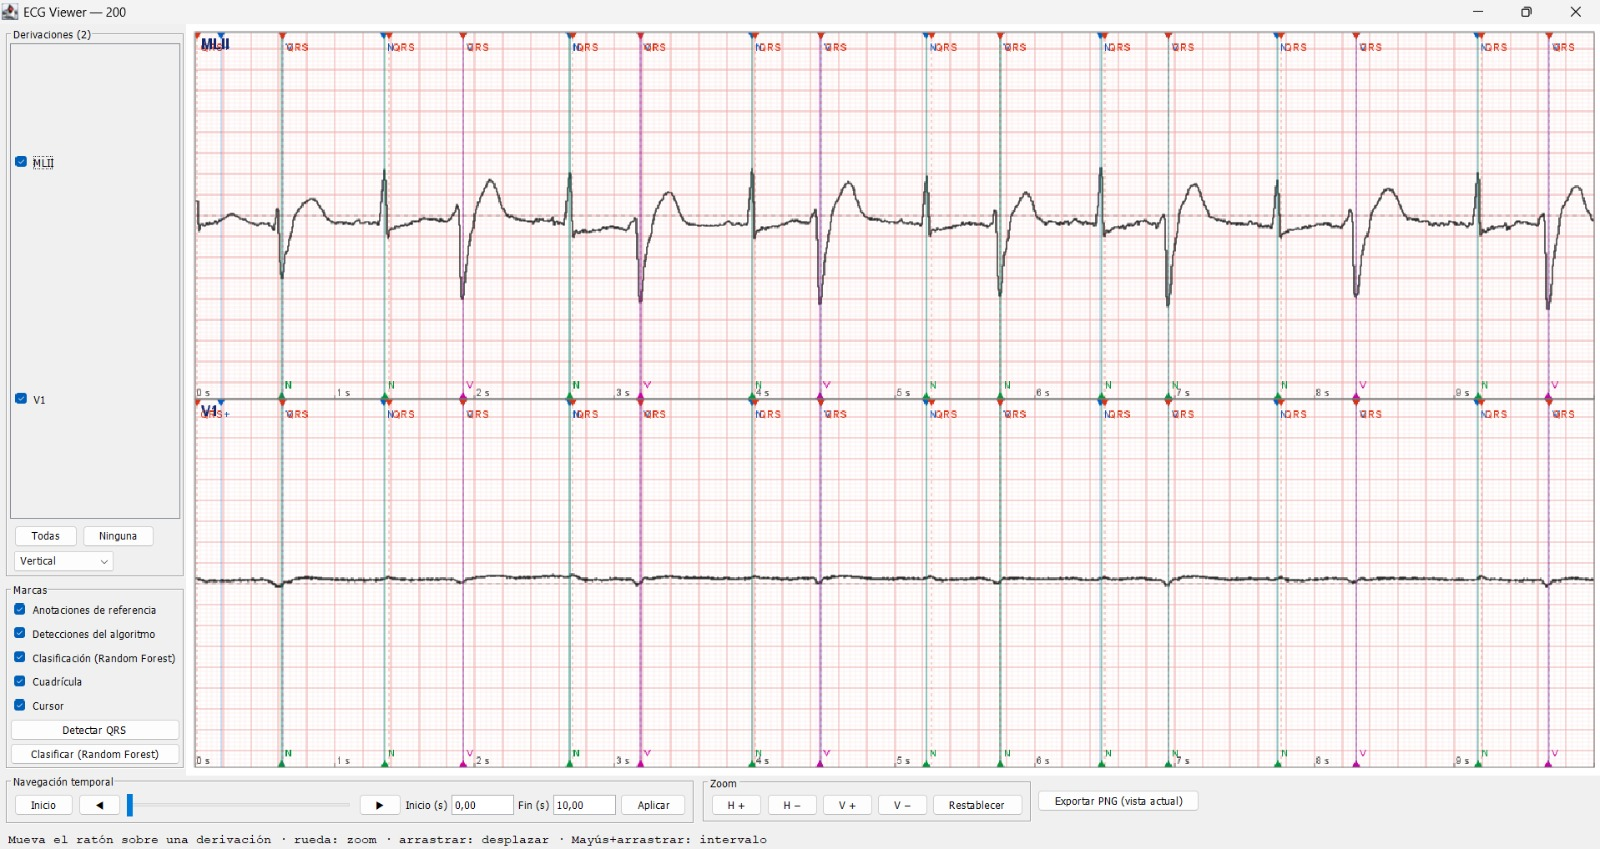
\includegraphics[width=\columnwidth]{images/gui.png}
\caption{Visor interactivo: selección dinámica de derivaciones, controles de distribución, marcas, navegación temporal, zoom y lectura del cursor (tiempo, muestra, derivación y amplitud).}
\label{fig:gui}
\end{figure}




\section{Metodología experimental}
%=====================================================================

\textbf{Datos.} Se emplearon los repositorios públicos de PhysioNet
\cite{goldberger2000}: la \emph{MIT-BIH Arrhythmia Database}
\cite{moody2001} para la clasificación de latidos (4 clases AAMI: N, S,
V, F), y las bases PTB Diagnostic ECG (PTBDB) y PTB-XL \cite{wagner2020}
para validar la lectura de registros de 12 derivaciones con metadatos
heterogéneos. La partición de evaluación sigue la propuesta de de Chazal
et al.~\cite{dechazal2004} (DS1/DS2 por registro). Los registros de
MIT-BIH se leyeron directamente de los archivos \texttt{.hea}/\texttt{.dat}/\texttt{.atr}
con el lector WFDB descrito en la Sección~2; los de PTBDB y PTB-XL se
usaron para comprobar la conversión de unidades, la ganancia por canal y
el número variable de derivaciones. Adicionalmente, el generador
sintético incluido en el proyecto permitió verificar la cadena completa
(cabecera, formato 16/212, \emph{checksum} y anotaciones con SKIP) en
casos controlados.

\textbf{Experimento A (detección).} Se evaluó el detector Pan-Tompkins
por derivación y la fusión por consenso sobre registros reales de
MIT-BIH (360\,Hz, 2 derivaciones, formato 212) con tolerancia
$\tau=0{,}15$\,s, comparando contra las anotaciones de referencia del
\texttt{.atr}. La validación se realizó registro a registro.

%\textbf{Experimento B (escalabilidad).} Registros de 12 derivaciones a
%500\,Hz con duración de 30, 60, 120, 300 y 600\,s, en formatos 16 y 212.
%Para cada uno se midieron la carga completa (cabecera, validación,
%decodificación, conversión y anotaciones), la detección en las 12
%derivaciones con fusión y la generación de la impresión estándar de
%5\,s. Se realizaron dos repeticiones de calentamiento y cinco medidas,
%con recolección de basura previa a cada una; se informa la media.

\textbf{Campaña de 15 pruebas preliminares (esta entrega).} Con el
clasificador ya entrenado con DS1, se ejecutó el flujo completo
(carga $\rightarrow$ detección QRS $\rightarrow$ fusión $\rightarrow$
extracción de 257 características $\rightarrow$ clasificación con el
bosque $\rightarrow$ validación contra referencia) sobre 15 registros
de MIT-BIH: 200, 201, 202, 203, 205, 207, 208, 209, 210, 212, 213, 214,
215, 217 y 219. Cada prueba corresponde a un registro (P001--P015 en la
Tabla~\ref{tab:campana}) y se ejecutó en una sesión independiente de la
JVM. Para cada prueba se registraron: el número de latidos por clase en
la referencia (Soporte N/S/V/F), la matriz de confusión $4\times4$, las
métricas por clase (precisión, \emph{recall}, especificidad, $F_1$) y
las métricas globales (\emph{accuracy}, $F_1$ macro, \emph{balanced
accuracy}), además de los tiempos y el consumo de recursos de cada
operación del flujo (carga, decodificación, análisis QRS, clasificación
RF, apertura del visor y exportación PNG). La Tabla~\ref{tab:campana}
resume los resultados de clasificación; la Tabla~\ref{tab:tiempos}
resume los tiempos y el heap máximo por operación, promediados sobre las
15 pruebas. Los informes PDF individuales
(\texttt{informe\_rendimiento\_*.pdf}) se generaron con el módulo de
rendimiento descrito en la Sección~\ref{sec:rend}.

%\textbf{Entorno.} Las pruebas de clasificación y de rendimiento de esta
%entrega se ejecutaron en Windows~11 (amd64) con 20 procesadores,
%OpenJDK~25.0.4.1 (Eclipse Adoptium) y \texttt{-Xmx2g}. El experimento B
%de escalabilidad se ejecutó en Linux~6.18 (amd64), OpenJDK~21.0.12, un
%único procesador y 4\,GB de RAM, en modo sin pantalla; por tanto, sus
%tiempos no son directamente comparables con los de la
%Tabla~\ref{tab:tiempos}. La verificación de la generación de PDF se
%realizó con PDFBox~2.0.29; el código está escrito para la serie 3.x
%declarada en el \texttt{pom.xml} (solo difiere la creación de las
%fuentes).

\textbf{Pruebas automáticas.} 31 pruebas JUnit~5 cubren la lectura
(cabeceras, formatos 16/212/8/24/32 con vectores construidos a mano,
conversión de unidades, anotaciones con SKIP, \emph{checksum}, ausencia
de ganancia), el procesamiento (detección, fusión, validación, RR/FC),
la visualización (distribuciones, zoom con punto fijo, selección y
cursor), la exportación (calibración exacta, coincidencia píxel a píxel
con la pantalla, paginación) y el rendimiento (medidores, anidamiento,
PDF y evaluación experimental).

\section{Resultados}
%=====================================================================

\subsection{Detección de QRS sobre MIT-BIH}
En los 15 registros evaluados (Sección~5), la fusión por consenso de las
dos derivaciones alcanzó $Se=P^{+}=F_1\approx 1{,}000$ frente a las
anotaciones de referencia, con un error temporal medio inferior a una
muestra a 360\,Hz. El número de latidos emparejados por registro varió
entre 405 (registro 217, con abundantes latidos de la clase V) y 3\,355
(registro 215), cubriendo un total de 39\,773 latidos emparejados en el proceso. Los detalles por registro están en el informe de rendimiento
individual de cada prueba.

\subsection{Clasificación de latidos (15 pruebas preliminares)}
La Tabla~\ref{tab:campana} resume el desempeño del bosque aleatorio
sobre los 15 registros de MIT-BIH. El \emph{accuracy} global osciló
entre 0,789 (registro 214) y 0,997 (registro 212), con una mediana de
0,945. La clase N se predijo con precisión y \emph{recall} superiores a
0,95 en la mayoría de los registros; la clase V se detectó con
\emph{recall} alto (0,85--1,00) cuando había suficientes ejemplos de
entrenamiento, pero su precisión cayó en registros con morfologías
atípicas (p.\,ej., 214: precisión 0,197 con 517 predicciones V frente a
138 reales). Las clases S y F son las más difíciles: S tiene soportes
pequeños (0--383 latidos) y el bosque tiende a predecir N; F solo
aparece en el registro 208 (353 latidos), donde el \emph{recall} fue
0,448. La \emph{balanced accuracy} (media de \emph{recall} por clase)
osciló entre 0,29 (registro 210) y 0,997 (registro 212); esta métrica
refleja mejor que el \emph{accuracy} el desbalance severo entre clases
(N y V concentran $>90\ porciento$ de los latidos en la mayoría de los
registros).

\begin{table*}[t]
\centering\footnotesize
\caption{Procedimiento de 15 pruebas preliminares sobre MIT-BIH (2
derivaciones, 360\,Hz, bosque de 200 árboles). Se muestran los soportes
por clase en la referencia, las métricas globales y el $F_1$ por clase.
Los registros con soporte 0 en una clase no permiten calcular su
$F_1$ (se indica con «--»).}
\label{tab:campana}
\begin{tabular}{@{}lrrrrrrrrrrrr@{}}
\toprule
 & \multicolumn{4}{c}{Soporte} & \multicolumn{3}{c}{Global} & \multicolumn{4}{c}{$F_1$ por clase}\\
\cmidrule(lr){2-5}\cmidrule(lr){6-8}\cmidrule(lr){9-12}
Reg. & N & S & V & F & Acc. & $F_1$ macro & Bal. acc. & N & S & V & F\\
\midrule
200 & 1742 & 30 & 794 & 2 & 0,942 & 0,470 & 0,463 & 0,959 & 0,000 & 0,921 & 0,000\\
201 & 1635 & 105 & 18 & 0 & 0,945 & 0,529 & 0,680 & 0,971 & 0,174 & 0,971 & --\\
202 & 2060 & 55 & 11 & 1 & 0,970 & 0,380 & 0,341 & 0,985 & 0,000 & 0,533 & 0,000\\
203 & 2491 & 2 & 409 & 1 & 0,975 & 0,473 & 0,458 & 0,986 & 0,000 & 0,908 & 0,000\\
205 & 2570 & 3 & 71 & 11 & 0,992 & 0,486 & 0,475 & 0,996 & 0,000 & 0,948 & 0,000\\
207 & 1540 & 107 & 181 & 0 & 0,973 & 0,694 & 0,875 & 0,984 & 0,856 & 0,935 & --\\
208 & 1579 & 2 & 944 & 353 & 0,931 & 0,639 & 0,612 & 0,944 & 0,000 & 0,994 & 0,617\\
209 & 2620 & 383 & 1 & 0 & 0,895 & 0,311 & 0,393 & 0,943 & 0,302 & 0,000 & --\\
210 & 2421 & 20 & 179 & 9 & 0,932 & 0,311 & 0,291 & 0,964 & 0,000 & 0,279 & 0,000\\
212 & 2746 & 0 & 0 & 0 & 0,997 & 0,250 & 0,997 & 0,998 & -- & -- & --\\
213 & 2640 & 28 & 158 & 361 & 0,877 & 0,403 & 0,497 & 0,959 & 0,000 & 0,653 & 0,000\\
214 & 2001 & 0 & 138 & 1 & 0,789 & 0,297 & 0,511 & 0,875 & -- & 0,311 & 0,000\\
215 & 3188 & 3 & 163 & 1 & 0,968 & 0,377 & 0,339 & 0,983 & 0,000 & 0,525 & 0,000\\
217 & 244 & 0 & 161 & 0 & 0,844 & 0,411 & 0,804 & 0,886 & -- & 0,757 & --\\
219 & 2082 & 7 & 58 & 1 & 0,991 & 0,473 & 0,453 & 0,995 & 0,000 & 0,895 & 0,000\\
\bottomrule
\end{tabular}
\end{table*}

\begin{table*}[t]
\centering\footnotesize
\caption{Tiempos medios (ms) y heap máximo (MiB) por operación,
promediados sobre las 15 pruebas del muestreo (Windows~11, 20
procesadores, OpenJDK~25.0.4.1).}
\label{tab:tiempos}
\begin{tabular}{@{}lrrrr@{}}
\toprule
Operación & Media (ms) & Mín. (ms) & Máx. (ms) & Heap máx. (MiB)\\
\midrule
Leer cabecera & 0,41 & 0,29 & 0,54 & \emph{ver nota}\\
Decodificar señales & 35,6 & 25,1 & 59,9 & \emph{ver nota}\\
Leer anotaciones & 2,06 & 0,81 & 5,15 & \emph{ver nota}\\
Cargar registro & 45,3 & 29,2 & 77,4 & \emph{ver nota}\\
Analizar QRS & 51,6 & 34,2 & 140,9 & \emph{ver nota}\\
Clasificar latidos (RF) & 144,9 & 97,3 & 204,7 & \emph{ver nota}\\
Abrir visor & 30,4 & 22,3 & 135,9 & \emph{ver nota}\\
Exportar PNG & 37,2 & 32,9 & 67,3 & \emph{ver nota}\\
\bottomrule
\end{tabular}
\end{table*}

\emph{Nota:} el heap máximo de la Tabla~\ref{tab:tiempos} se informa en
el Excel por prueba y no por operación; los valores oscilaron entre
20,6\,MiB (P001, lectura de cabecera) y 837,7\,MiB (P006, análisis QRS),
con una tendencia creciente a lo largo de la sesión por acumulación de
referencias vivas entre pruebas (la JVM no se reinició entre P001 y
P015). El detalle por prueba está en el archivo
\texttt{resultados\_pruebas.xlsx} y en los informes PDF individuales.



\subsection{Ejemplo de informe de rendimiento}
La evaluación experimental de un registro de 60\,s y 12 derivaciones
(tres repeticiones tras el calentamiento) produjo un informe PDF de tres
páginas. Las operaciones de mayor coste fueron la exportación PNG de la
imagen estándar de $1\,891\times852$ píxeles (125\,ms de media) y su
renderizado (105\,ms), frente a 39\,ms para cargar el registro (de ellos
25\,ms de decodificación) y 28\,ms para la detección en las doce
derivaciones. En ese informe el heap máximo observado fue de 29,3\,MiB
mientras que la memoria residente fue de 103\,MiB, una diferencia de más
de tres veces que ilustra por qué ambas magnitudes se informan por
separado. En la plataforma Linux utilizada fue posible informar CPU de
usuario y de sistema; en Windows las columnas de CPU aparecen como «no
disponible» y solo se informa el heap (como en la
Tabla~\ref{tab:tiempos}).

% =========================================================
% AGRADECIMIENTOS
% =========================================================
%ESTO ENTRA PARA POSTERIORES ENTREGAS
%\section*{Agradecimientos}

%Los autores agradecen a la Universidad Nacional de Colombia, Sede Amazonia,
%y a las personas o instituciones que apoyaron el desarrollo de este proyecto.

% =========================================================
% REFERENCIAS
% Sin BibTeX ni Biber para reducir tiempo de compilación.
% =========================================================

\begin{thebibliography}{00}

%\bibitem{cormen}
%T. H. Cormen, C. E. Leiserson, R. L. Rivest y C. Stein,
%\textit{Introduction to Algorithms}, 4th ed.
%Cambridge, MA, USA: MIT Press, 2022.

\bibitem{pt}
School of Electrical and Computer Engineering  Cornell David A. Duffield College of Engineering. Accedido el 14 de octubre de 2026. [En línea]. Disponible: \url{https://people.ece.cornell.edu/land/courses/ece5030/labs/s2014/Pan_Tompkins.pdf}
\bibitem{MtECG}
A. J. Prakash, A. N. Belkacem, I. M. Elfadel, H. F. Jelinek y M. Atef. “Frontiers | Advances in machine and deep learning for ECG beat classification: a systematic review”. Frontiers. Accedido el 11 de noviembre de 2026. [En línea]. Disponible: https://www.frontiersin.org/journals/digital-health/articles/10.3389/fdgth.2025.1649923/full
\bibitem{MIT-BIH}
G. Moody and R. Mark, "MIT-BIH Arrhythmia Database," PhysioNet, version 1.0.0, feb. 2005. doi: 10.13026/C2F305
\bibitem{RF}
H. A. Salman, A. Kalakech, and A. Steiti, "Random Forest Algorithm Overview," Babylonian Journal of Machine Learning, vol. 2024, pp. 69-79, Jun. 2024, doi: 10.58496/BJML/2024/007.
\bibitem{interpretacionECG}
Kligfield P, Gettes LS, Bailey JJ, et al. Recommendations
for the standardization and interpretation of
the electrocardiogram. Circulation 2007;115(10):1306-1313.
\bibitem{PhysioNet}
Pollard, T., Moody, B. E., Lehman, L., Gow, B., Fernandes, C., Xie, C., Johnson, A., Mark, R. G., Heldt, T. (2026). PhysioNet as a global platform for biomedical research. Nature Health. https://doi.org/10.1038/s44360-026-00096-z. Available from: https://pmc.ncbi.nlm.nih.gov/articles/PMC13641116/
\bibitem{goldberger2000} Goldberger AL, Amaral LAN, Glass L, et al. PhysioBank, PhysioToolkit, and PhysioNet: components of a new research resource for complex physiologic signals. \emph{Circulation} 2000;101(23):e215--e220.
\bibitem{moody2001} Moody GB, Mark RG. The impact of the MIT-BIH Arrhythmia Database. \emph{IEEE Eng Med Biol Mag} 2001;20(3):45--50.
\bibitem{wagner2020} Wagner P, Strodthoff N, Bousseljot RD, et al. PTB-XL, a large publicly available electrocardiography dataset. \emph{Sci Data} 2020;7:154.
\bibitem{pantompkins1985} Pan J, Tompkins WJ. A real-time QRS detection algorithm. \emph{IEEE Trans Biomed Eng} 1985;32(3):230--236.
\bibitem{kligfield2007} Kligfield P, Gettes LS, Bailey JJ, et al. Recommendations for the standardization and interpretation of the electrocardiogram. \emph{Circulation} 2007;115(10):1306--1313.
\bibitem{wfdb} PhysioNet. WFDB Software Package: header and signal file specifications. \url{https://physionet.org/content/wfdb/}
\bibitem{pdfbox} Apache Software Foundation. Apache PDFBox. \url{https://pdfbox.apache.org/}
\bibitem{oraclejmx} Oracle. Java SE API: \texttt{java.lang.management} (\texttt{ThreadMXBean}, \texttt{OperatingSystemMXBean}).
% Breiman, L. (2001). Random Forests. Machine Learning, 45(1), 5-32.
% Quinlan, J. R. (1986). Induction of Decision Trees. Machine Learning, 1(1), 81-106.
 \bibitem{dechazal2004}
de Chazal, P., O'Dwyer, M., Reilly, R. B. (2004). Automatic Classification of Heartbeats Using ECG Morphology and Heartbeat Interval Features.
%   IEEE Trans. Biomedical Engineering, 51(7), 1196-1206.
\end{thebibliography}

\end{document}
